\section{Analyze attack trends}\label{analyze-attack-trends}

\begin{figure}[tb]

{\centering 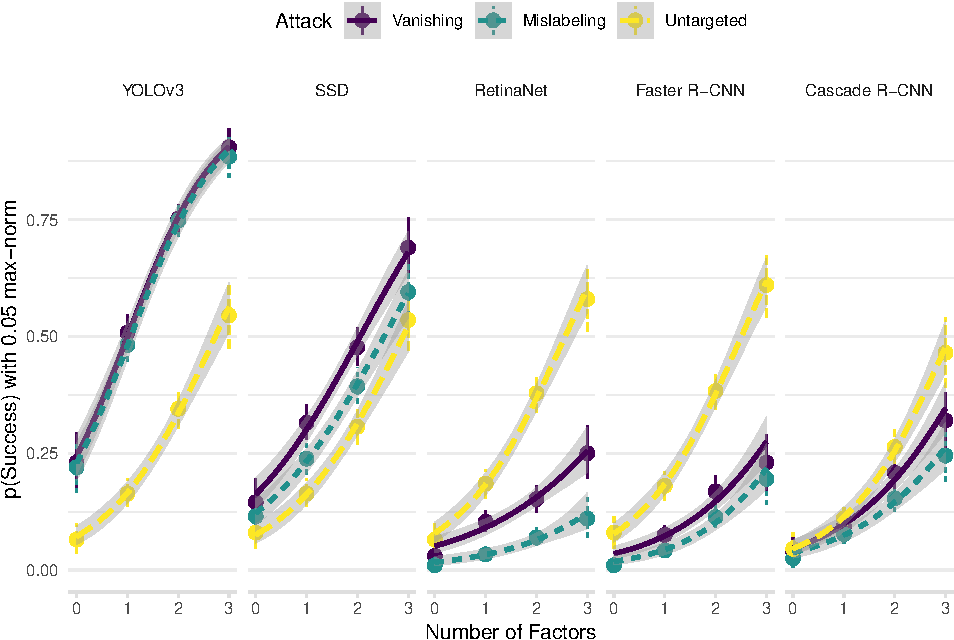
\includegraphics[width=1\linewidth]{imgs/biased_trend_graph_normed} 

}

\caption{\textbf{Success factors can be exploited in combination to significantly increase success rates even with 0.05 max-norm:}  We sampled target and perturb objects based on three validated success factors in Table \ref{tab:results_table} by targeting objects with low predicted confidence, perturbing large objects and selecting target and perturb objects close to one another. The binned summaries and regression trendlines graph success proportion against number of factors in the deliberate attack experiment. Errors are 95\% confidence intervals and every point aggregates success over 200 images. Success rates significantly increase as the number of factors combined increases. Significance is determined at $\alpha < 0.05$ using a Wald z-test on the logistic estimates. Full details are given in Section \ref{sec:del_per}.}\label{fig:biased_trend_graph_normed}
\end{figure}

\begingroup\fontsize{9}{11}\selectfont

\begin{longtable}[t]{llllrrrrrr}
\caption{\label{tab:num_cri_table}We run a logistic model regressing success against log(number of factors) in the randomized attack experiment. Success rates increase with the number of factors combined to select target and perturb objects for all models and attacks. Table headers are explained in Appendix \ref{app:tab_hdr}.}\\
\toprule
\multicolumn{2}{c}{Group} & \multicolumn{8}{c}{Regression} \\
\cmidrule(l{3pt}r{3pt}){1-2} \cmidrule(l{3pt}r{3pt}){3-10}
 & Attack & term & sig & estimate & std.error & statistic & p.value & conf.low & conf.high\\
\midrule
\addlinespace[0.3em]
\multicolumn{10}{l}{\textbf{YOLOv3}}\\
\hspace{1em} & Vanishing & num\_cri & * & 1.132 & 0.075 & 15.133 & 0 & 0.987 & 1.281\\
\cmidrule{2-10}\nopagebreak
\hspace{1em} & Mislabeling & num\_cri & * & 1.134 & 0.074 & 15.240 & 0 & 0.991 & 1.283\\
\cmidrule{2-10}\nopagebreak
\hspace{1em} & Untargeted & num\_cri & * & 0.938 & 0.076 & 12.307 & 0 & 0.791 & 1.090\\
\cmidrule{1-10}\pagebreak[0]
\addlinespace[0.3em]
\multicolumn{10}{l}{\textbf{SSD}}\\
\hspace{1em} & Vanishing & num\_cri & * & 0.800 & 0.067 & 11.974 & 0 & 0.671 & 0.933\\
\cmidrule{2-10}\nopagebreak
\hspace{1em} & Mislabeling & num\_cri & * & 0.781 & 0.069 & 11.291 & 0 & 0.647 & 0.919\\
\cmidrule{2-10}\nopagebreak
\hspace{1em} & Untargeted & num\_cri & * & 0.864 & 0.076 & 11.408 & 0 & 0.718 & 1.015\\
\cmidrule{1-10}\pagebreak[0]
\addlinespace[0.3em]
\multicolumn{10}{l}{\textbf{RetinaNet}}\\
\hspace{1em} & Vanishing & num\_cri & * & 0.615 & 0.091 & 6.760 & 0 & 0.439 & 0.795\\
\cmidrule{2-10}\nopagebreak
\hspace{1em} & Mislabeling & num\_cri & * & 0.703 & 0.137 & 5.131 & 0 & 0.438 & 0.976\\
\cmidrule{2-10}\nopagebreak
\hspace{1em} & Untargeted & num\_cri & * & 0.956 & 0.075 & 12.780 & 0 & 0.812 & 1.105\\
\cmidrule{1-10}\pagebreak[0]
\addlinespace[0.3em]
\multicolumn{10}{l}{\textbf{Faster R-CNN}}\\
\hspace{1em} & Vanishing & num\_cri & * & 0.783 & 0.097 & 8.062 & 0 & 0.595 & 0.976\\
\cmidrule{2-10}\nopagebreak
\hspace{1em} & Mislabeling & num\_cri & * & 0.903 & 0.117 & 7.729 & 0 & 0.678 & 1.136\\
\cmidrule{2-10}\nopagebreak
\hspace{1em} & Untargeted & num\_cri & * & 0.985 & 0.075 & 13.115 & 0 & 0.840 & 1.135\\
\cmidrule{1-10}\pagebreak[0]
\addlinespace[0.3em]
\multicolumn{10}{l}{\textbf{Cascade R-CNN}}\\
\hspace{1em} & Vanishing & num\_cri & * & 0.794 & 0.088 & 9.069 & 0 & 0.625 & 0.968\\
\cmidrule{2-10}\nopagebreak
\hspace{1em} & Mislabeling & num\_cri & * & 0.743 & 0.097 & 7.689 & 0 & 0.556 & 0.936\\
\cmidrule{2-10}\nopagebreak
\hspace{1em} & Untargeted & num\_cri & * & 0.982 & 0.084 & 11.703 & 0 & 0.820 & 1.149\\
\bottomrule
\end{longtable}
\endgroup{}
